We present two independent validations of the analysis pipeline. The first of them is based on a detailed simulation of the observation of a tSZ cluster with known physical parameters and typical atmospheric and electronic noise. The second one is based on the observation of a faint cluster that allow us to show that the tSZ detection is not an artifact of the data analysis and/or acquisition. 

 \subsection{Simulation}
 \label{sec:simu}	
To test the pipeline as described in Sect.~\ref{sec:SZ_analysis}, we simulate the {\it NIKA} observations of a cluster and construct the TODs by taking all terms of Eq.~\ref{eq:signal_and_noise} into account, which includes the atmospheric contamination, the electronic noise, and the tSZ signal. The parameters used in the simulation are given in Table~\ref{tab:table_param_simu} and are representative of the weather conditions for the observations described in this paper.
\begin{table}
\begin{center}
\begin{tabular}{cc}
\hline
\hline
Parameter & Value \\
\hline
$v_{\mathrm{H}_2\mathrm{O}}$ & 1 \ m/s\\
$h_{\mathrm{H}_2\mathrm{O}}$ & 3000 \ m \\
$\alpha_{\mathrm{H}_2\mathrm{O}}$ & -1.35 \\
$\tau_{140 \ \mathrm{GHz}}$ & 0.1 \\
$\tau_{240 \ \mathrm{GHz}}$ & 0.12 \\
$\left({F_{\mathrm{H}_2\mathrm{O}}}\right)_{140 \ \mathrm{GHz}}$ & 28 \ Jy/beam \\
$\left({F_{\mathrm{H}_2\mathrm{O}}}\right)_{240 \ \mathrm{GHz}}$ & 110 \ Jy/beam \\
$F_{\mathrm{el}} (140 \ \mathrm{GHz})$ & 14 \ Jy/beam/K \\
$F_{\mathrm{el}} (240 \ \mathrm{GHz})$ & 35 \ Jy/beam/K \\
$T_{\mathrm{atmo}}$ & 233 \ K \\
$E_0(1 \ \mathrm{Hz,} \ 140 \ \mathrm{GHz})$ & 38 \ mJy/beam \\
$E_0(1 \ \mathrm{Hz,} \ 240 \ \mathrm{GHz})$ & 76 \ mJy/beam \\
$\beta$ & -0.25 \\ 
$N_0 (140 \ \mathrm{GHz})$ & 29 \ $\mathrm{mJy.s}^{1/2}$ \\
$N_0 (240 \ \mathrm{GHz})$ & 57 \ $\mathrm{mJy.s}^{1/2}$ \\ 
$R_{\mathrm{g}}$ & 0.065 s$^{-1}$ \\
\hline
\end{tabular}
\end{center}
\caption{Values of the parameters used in the simulation; see text for details.}
\label{tab:table_param_simu}
\end{table}

 \subsubsection{Atmospheric contribution}
 \label{sec:atmo_simu}
 The atmospheric contribution $A(\nu_b, t)$ is simulated as described in Sect.~\ref{sec:SZ_analysis}.

The water vapor fluctuations ({\it i.e.}, $a_{\mathrm{H}_2\mathrm{O}} ^{\mathrm{fluc}} \times A_{\mathrm{H}_2\mathrm{O}}^{\mathrm{fluc}} (t)$) are obtained by simulating a map of water vapor anisotropy that passes in front of the telescope aperture with a speed $v_{\mathrm{H}_2\mathrm{O}}$ at an altitude $h_{\mathrm{H}_2\mathrm{O}}$ above the telescope. The power spectrum of this map is a power law with slope $\alpha_{\mathrm{H}_2\mathrm{O}}$. The amplitudes of the atmospheric fluctuations are then normalized to have a standard deviation over the time of the scan equal to $\sigma = F_{\mathrm{H}_2\mathrm{O}} \left(1-\mathrm{exp} \left(-\frac{\tau}{\mathrm{sin} (el)}\right) \right)$, where $\tau$ is the zenith opacity, $el$ the elevation, and $F_{\mathrm{H}_2\mathrm{O}}$ is the reference flux. 

The contribution of the elevation terms, both from $\mathrm{H}_2\mathrm{O}$ and $\mathrm{O}_2$, is simulated as 
   \begin{equation}
	  d_{\mathrm{el}}(t)~=~F_{\mathrm{el}} T_{\mathrm{atmo}} \left(\mathrm{exp}\left(-\frac{\tau}{\mathrm{sin}(<el>)}\right) - \mathrm{exp}\left(-\frac{\tau}{\mathrm{sin}(el)}\right)\right).
	\label{eq:el_term}
   \end{equation}
The parameter $T_{\mathrm{atmo}}$ is the temperature of the atmosphere, and $F_{\mathrm{el}}$ is a reference flux that is measured at both frequencies using skydips.

 \subsubsection{Electronic noise}
 \label{sec:elec_simu}
The electronic noise $E(\nu_b, t)$ is simulated as a common mode with a power spectrum slope $\beta$ and an amplitude $E_0$. This common-mode is identical for all detectors in a given frequency band but differs for the two bands since the electronics is not the same. The spectrum slope is the same for the two bands, but the amplitude is higher at 240~GHz than at 140~GHz (see Table~\ref{tab:table_param_simu}).
 
 \subsubsection{Uncorrelated noise}
 \label{sec:white_simu}
We also simulate a total uncorrelated noise term, $N_k(t)$, independently for each detector. This term accounts for various white noise contributions, including  photon noise, spontaneous Cooper pair breaking due to thermal noise fluctuations and electronic white noise. For the purpose of the simulations, we keep this noise contribution independent of the observing conditions. However, for the real observations, we find that the white noise level is coupled to the atmospheric conditions. This is mainly due to the broadening of the resonances for large optical loads, and it is not accounted for in the simulations. Similarly, we do not account for photon noise variations induced by changes in the optical load. For the sake of simplicity, the total root mean square of the uncorrelated noise is assumed to be identical for all detectors of the same array.
	
\subsubsection{Glitches}
\label{sec:glitch_simu}
Glitches are simulated with a rate $R_{\mathrm{g}}$. They only affect individual samples in the TODs ({\it i.e.}, the KID response is much faster than the sampling frequency) and simultaneously affect all KIDs of a given array ({\it i.e.}, glitches are assumed to generate phonons that hit all the KIDs of the array). The amplitudes of the glitches are generated using a Gaussian spectrum with a standard deviation of 1.3~Jy/beam, as observed in the measured TODs.
		
  \subsubsection{Pulse tube lines}
 \label{sec:ptl_simu}
To simulate the frequency lines generated by the pulse tube, we add cosine functions to the timeline that correspond to the typical frequencies and amplitudes seen in the data (see the power spectrum of the raw data in Fig.~\ref{fig:TOI_PS_real}).
   
\subsubsection{The thermal Sunyaev Zel'dovich signal}
 \label{sec:sz_simu}
       	\begin{table}
	\begin{center}
	\begin{tabular}{llccc}
	\hline
	\hline
	 & Compact cluster & Diffuse cluster \\
	\hline
	$\alpha$ & 1.2223 & 1.2223 \\
	$\beta$ & 5.4905 & 5.4905 \\
	$\gamma$ & 0.7736 & 0.7736 \\
	$r_{\mathrm{s}}$ (kpc) & 383 & 800 \\
	$\theta_{\mathrm{s}}$ (arcmin) & 1.1 & 2.3 \\
	$P_0 \ (\mathrm{keV/cm}^3)$ & 0.5 & 0.18 \\
	Best fit $\theta_{\mathrm{s}}$ (arcmin) & $1.048 \pm 0.042$ & $2.019 \pm 0.075$ \\   
	Best fit $P_0 \ (\mathrm{keV/cm}^3)$ & $0.449 \pm 0.052$ & $0.150 \pm 0.010$ \\  
	\hline
	\end{tabular}
	\end{center}
	\caption{Generalized Navarro, Frenk, and White parameters used to simulate the compact and diffuse clusters. The choice of the slope parameters is given in Sect.~\ref{sec:mcmc}. The last two lines provide the recovered marginalized best fit profile of the simulated clusters.}
	\label{tab:table_simu}
	\end{table}	
We use the generalized Navarro, Frenk, and White (gNFW) pressure profile \citep{gNFW} to describe the cluster pressure distribution out to a significant fraction of the virial radius. This profile is given by
\begin{equation}
	P(r) = \frac{P_0}{\left(\frac{r}{r_{\mathrm{s}}}\right)^{\gamma}\left(1+\left(\frac{r}{r_{\mathrm{s}}}\right)^{\alpha}\right)^{\frac{\beta-\gamma}{\alpha}}},
	\label{eq:gNFW}
   \end{equation}
where $P_0$ is a normalizing constant; $\alpha$, $\beta$, and $\gamma$ set the slope at intermediate, large, and small radii respectively, and $r_{\mathrm{s}}$ is the characteristic radius. The same profile can be written in its universal form \citep{arnaud_2010} by relating the characteristic radius to the concentration parameter $c_{500}$, $r_{\mathrm{s}} = r_{500}/c_{500}$, with $r_{500}$ the radius within which the mean density of the cluster is equal to 500 times the critical density of the Universe at the cluster redshift. The pressure normalization can then be written as $P_0 = P_{500} \times \mathds{P}_0$, where $\mathds{P}_0$ is a normalization factor and $P_{500}$ is the average pressure within the radius $r_{500}$ (related to the average mass within the same radius, $M_{500}$, by a scaling law). We finally define $\theta_{\mathrm{s}} = r_{\mathrm{s}}/D_A$ the characteristic angular size, where $D_A$ is the angular diameter distance of the cluster.

We simulate two different kinds of clusters. The first one is similar to what we observe for \mbox{RX~J1347.5-1145} in terms of amplitude and spatial extension (referred to as compact in the following). The second one is more diffuse, but its peak amplitude is the same as for the previous (referred to as diffuse hereafter). The corresponding parametrization can be found in Table~\ref{tab:table_simu}. Using these sets of parameters, we compute the Compton parameter map according to Eq.~(\ref{eq:y_compton}) by integrating the pressure along the line-of-sight. The map is then convolved with the instrumental beam and converted into surface brightness. We use the same scanning strategy, as in the case of \mbox{RX~J1347.5-1145} observations of {\it NIKA} during the Run 5. The focal plane and the number of detectors are also the same. The clusters are centered at the tSZ signal maximum decrement that we observe on \mbox{RX~J1347.5-1145}.

 \subsubsection{Validation of the pipeline on simulated data}
 \label{sec:valid_pipe_simu}
After processing the simulated data, we recover the two cluster maps (compact is labeled C and diffuse is labeled D). Figure \ref{fig:rxj_simu_map} provides the input model maps, the recovered maps after the processing, the residual between the input models and the recovered maps, and the best fit models of the recovered maps. The top line corresponds to the compact cluster and the second to the diffuse cluster. The clusters are detected with a signal-to-noise of the order of 10 and are well mapped in both cases. The signal amplitude is slightly reduced with respect to the input maps.
	\begin{figure*}
	\centering
	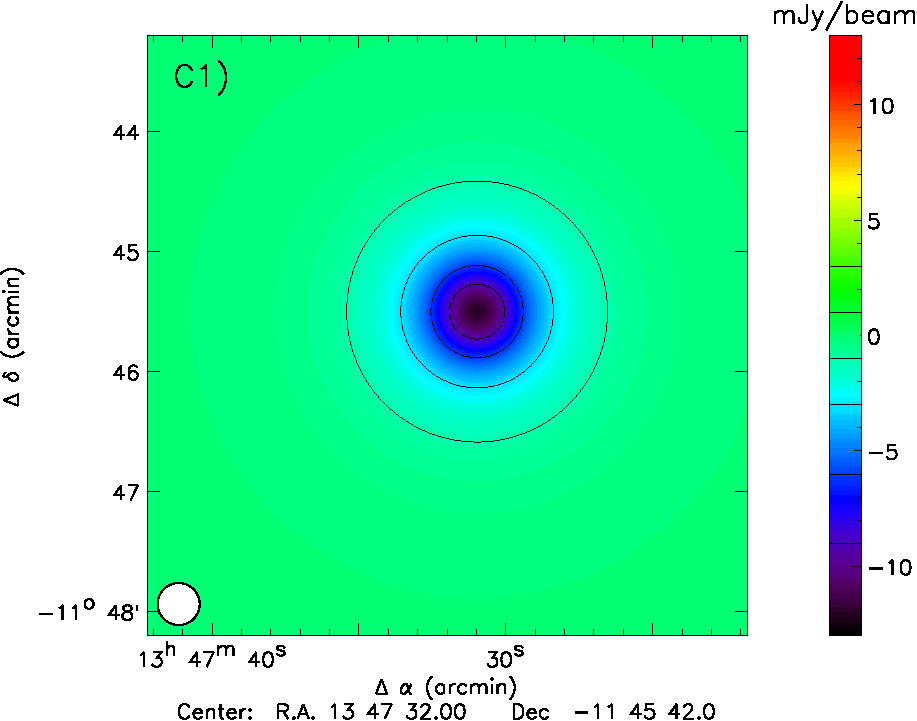
\includegraphics[width=4.5cm]{Figure/Simulation_RXJ1347_model_compact}
	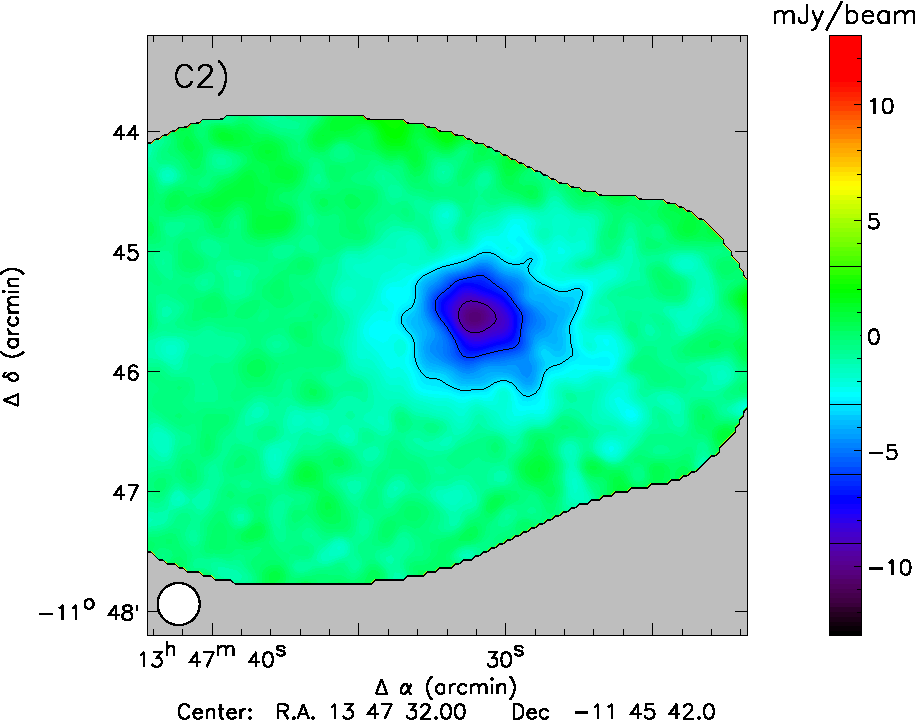
\includegraphics[width=4.5cm]{Figure/Simulation_RXJ1347_compact}
	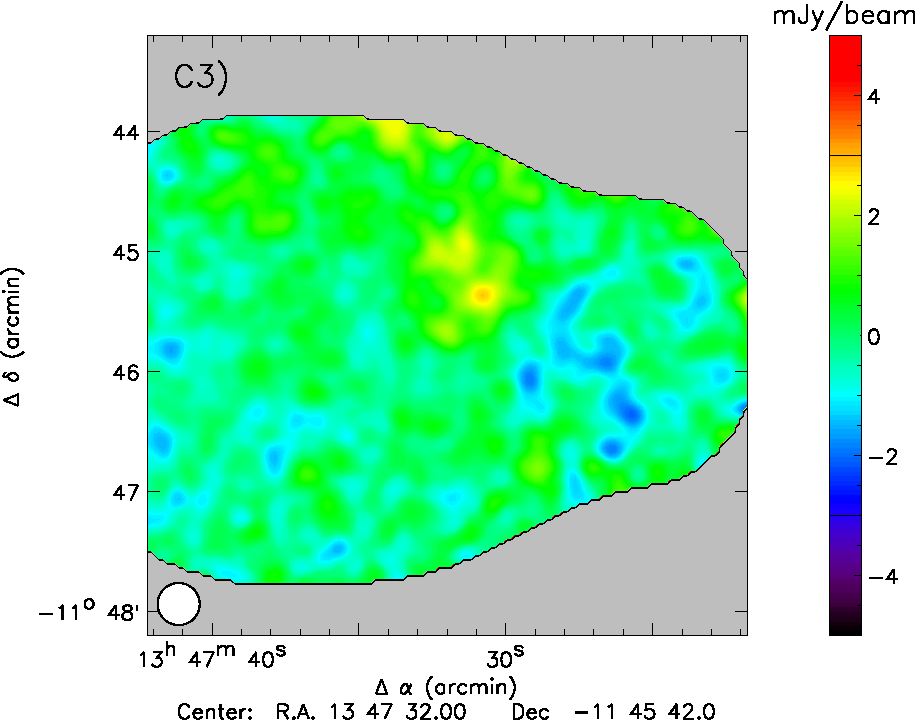
\includegraphics[width=4.5cm]{Figure/Simulation_RXJ1347_resi_compact}
	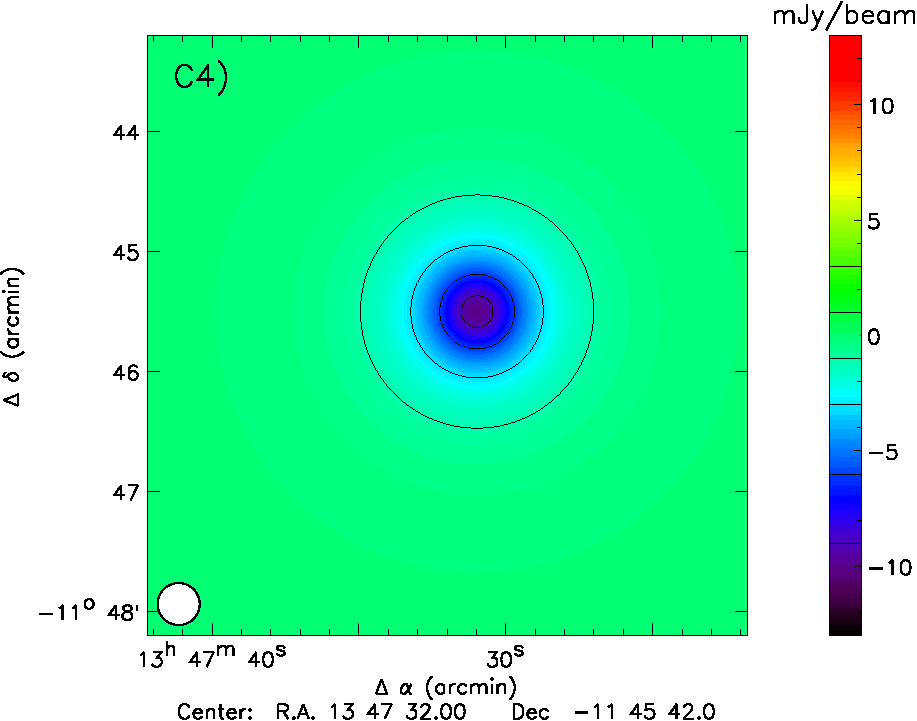
\includegraphics[width=4.5cm]{Figure/Simulation_RXJ1347_bestfit_compact}	
	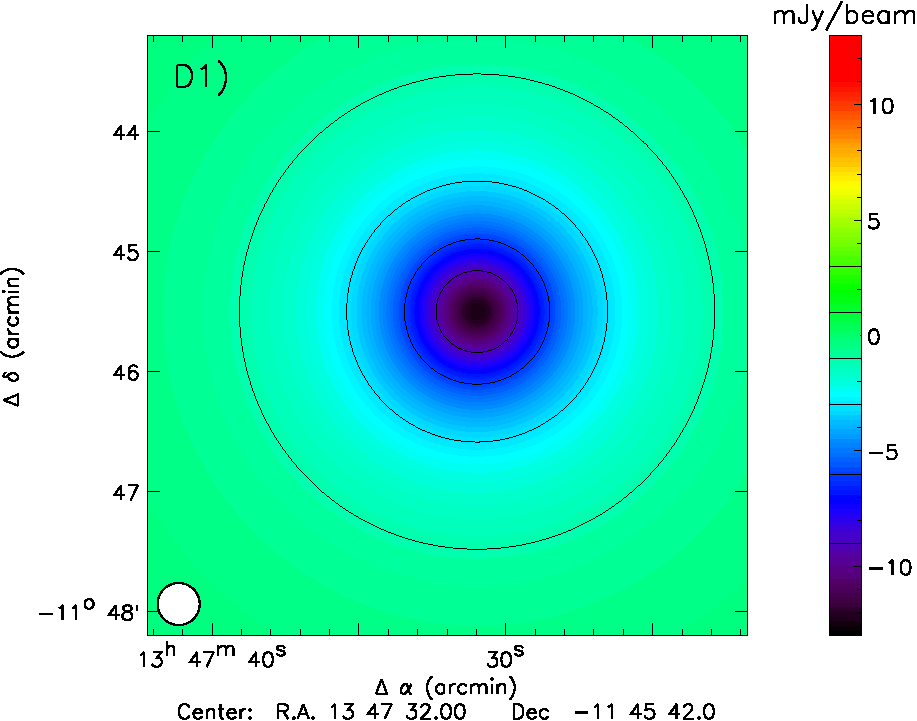
\includegraphics[width=4.5cm]{Figure/Simulation_RXJ1347_model_diffus}
	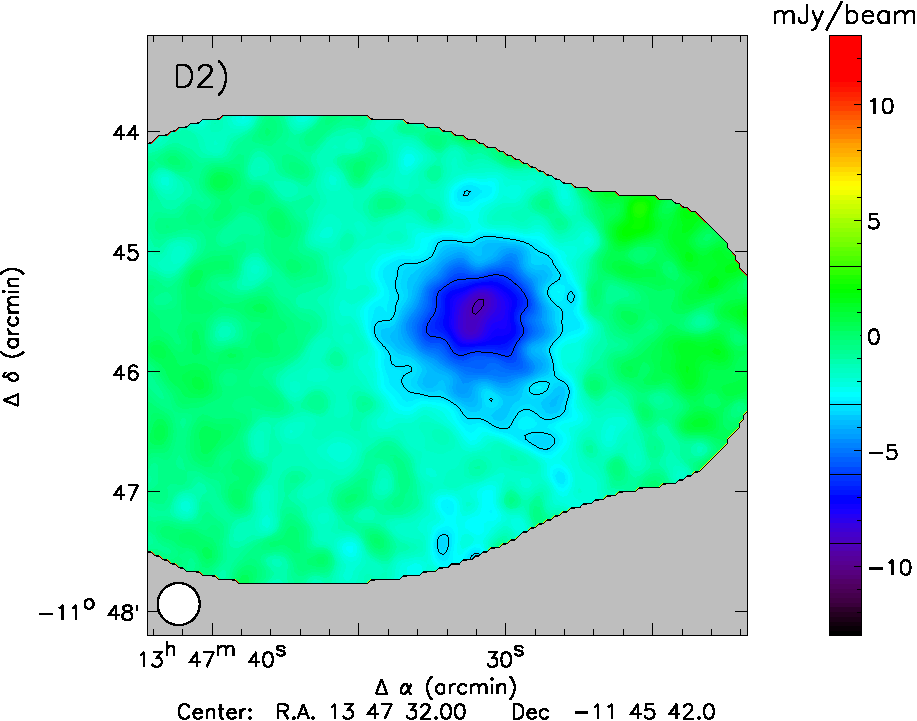
\includegraphics[width=4.5cm]{Figure/Simulation_RXJ1347_diffus}
	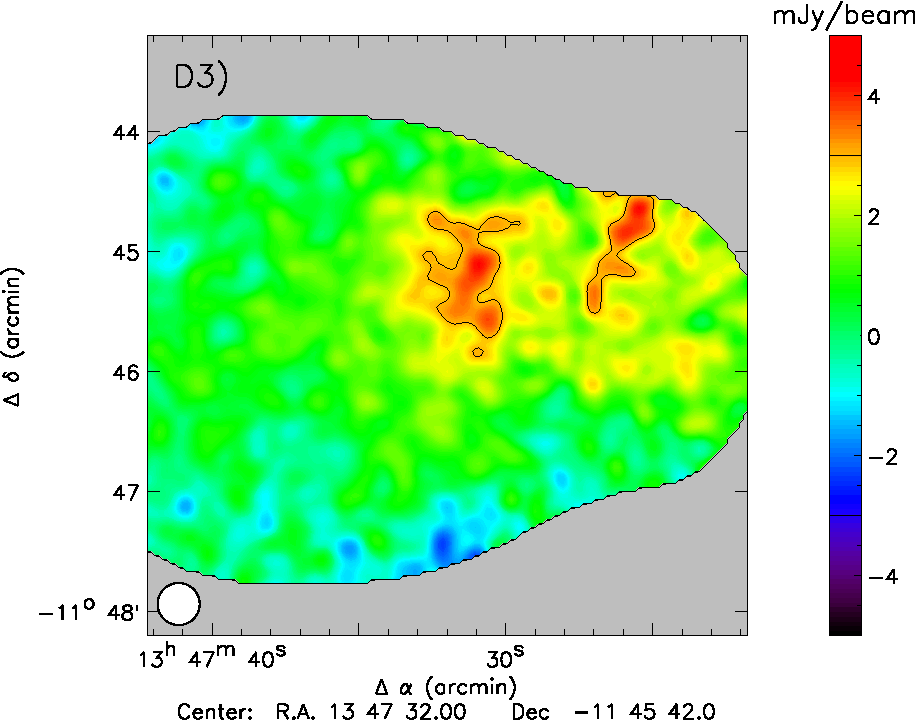
\includegraphics[width=4.5cm]{Figure/Simulation_RXJ1347_resi_diffus}
	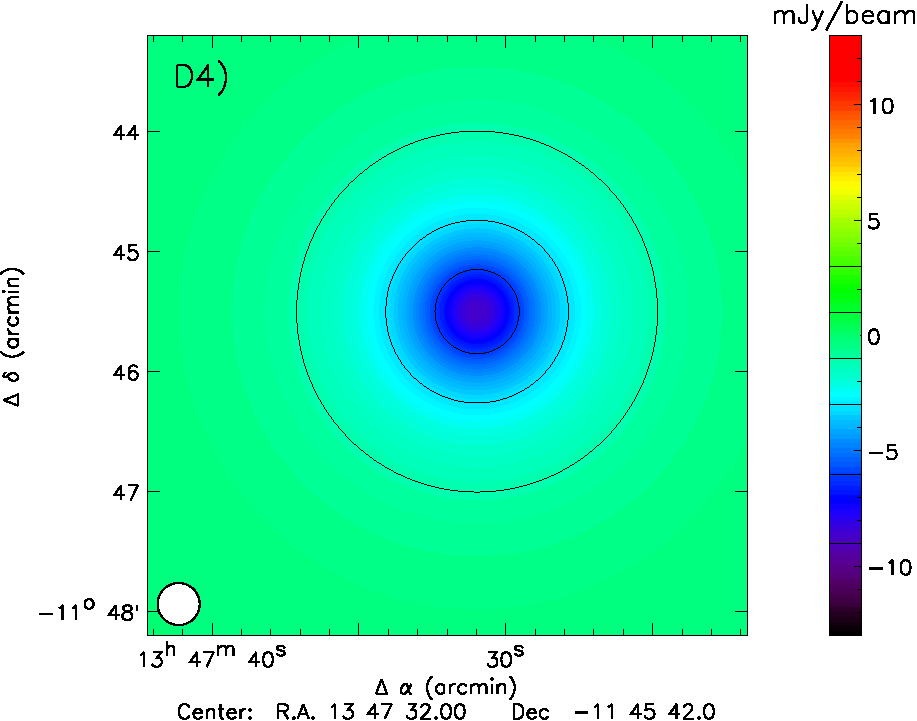
\includegraphics[width=4.5cm]{Figure/Simulation_RXJ1347_bestfit_diffus}
	\caption{Generalized Navarro, Frenk, and White simulations of two clusters processed through the pipeline. The first one (compact cluster, as C) is similar to the {\it NIKA} map of \mbox{RX~J1347.5-1145} (top panels). The second (diffuse cluster, labeled D) is more extended (bottom panels). The parameters used in the cluster simulations are given in Table~\ref{tab:table_simu}. From left to right, we show the input model maps, the recovered maps, the residual maps, and the best fit model maps of the recovered signal. They are labeled from C1 to C4 and from D1 to D4 for the compact and diffuse cluster, respectively. The maps are shown up to a noise level that is twice the minimal noise level of the map. The effective beam is shown on the bottom left corner, accounting for the instrumental beam and an extra 10~arcsec Gaussian smoothing of the maps. The contours correspond to  3, -3, -6, and -9 mJy/beam, to which we add -1 mJy/beam for the model maps. The color scales range from -13 to 13 mJy/beam, except for the residual maps for which we have -5 to 5 mJy/beam. The center of the clusters has been simulated at the tSZ peak location of the {\it NIKA}  \mbox{RX~J1347.5-1145} map.}
        \label{fig:rxj_simu_map}
	\end{figure*}

Using these maps, we compute the angular profiles of the recovered clusters by evaluating the average flux value for a set of concentric annuli. They are shown in Fig.~\ref{fig:rxj_simu_prof}, as green and red dots for the compact and diffuse clusters, respectively. Comparison with the input profiles is provided by solid lines with similar colors. We also show the profiles recovered after projection only  to check zero-level effects (orange and blue diamonds for the compact and diffuse cluster, respectively), that is the input tSZ signal is simply projected without decorrelation or filtering.
	\begin{figure}
	\centering
	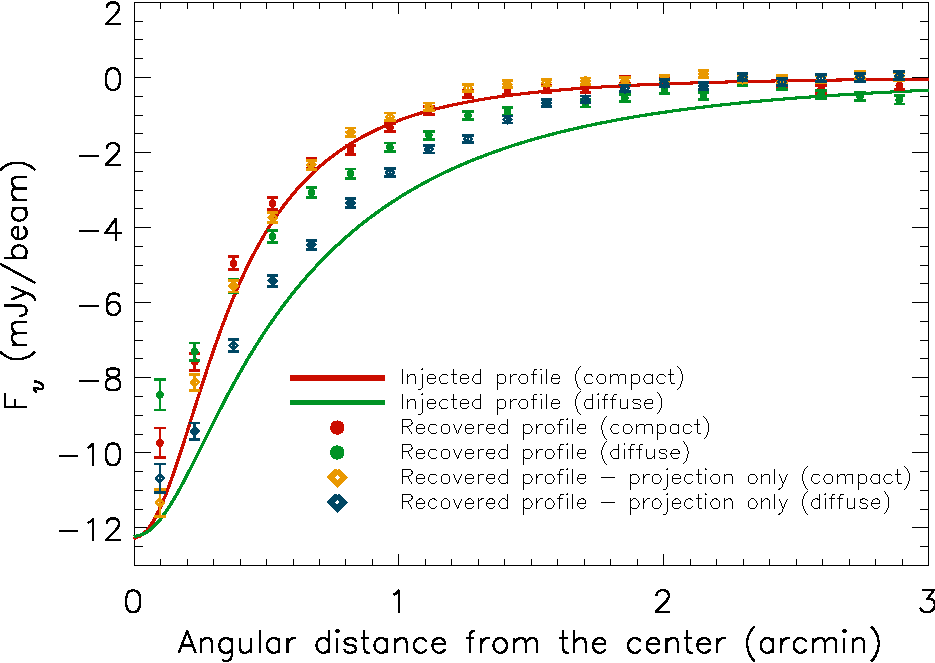
\includegraphics[width=\columnwidth]{Figure/pipeline_transfer}
	\caption{Comparison of the profiles injected in the simulation and recovered at the end of the pipeline. The injected profiles are given as red (compact cluster) and green (diffuse cluster) solid lines. The recovered profiles are shown with dots of similar colors. We also show the recovered profiles in the case of projection only without correlated noise, glitches, or pulse tube lines included in the simulation. They are given as orange (compact cluster) and blue (diffuse cluster) diamonds.}
        \label{fig:rxj_simu_prof}
	\end{figure}
	
First of all, due to the scanning strategy, the largest angular scale that can be recovered in the map is 6~arcmin, which corresponds to the size of the observed map. In Fig.~\ref{fig:rxj_simu_prof}, we show the profile of the diffuse cluster (projection only, as blue diamonds) that reaches the zero-level at 3~arcmin, which is unlike the injected profile that extends farther. Hence, the data processing affects the map in the case of the diffuse cluster by reducing the measured flux up to 25\% at a radii of $\sim~1$~arcmin. This can also be observed on the residual map of the diffuse cluster that is positive around the cluster peak. In the case of the compact cluster, the amplitude of the profile is not affected by more than 10\%, and the corresponding residual map is consistent with noise. Concerning the shape of the reconstructed signal with respect to the input one, we observe a flat transfer function for angular scales between  0.4 and 4~arcmin for the compact cluster case. Finally, the remaining correlated noise can slightly contaminate the profile, but it is not significant once averaged on concentric annuli.

We use the simulated maps to fit the normalization $P_0$ and the characteristic radius $r_{\mathrm{s}}$ of the pressure profile. This is done using Markov Chain Monte Carlo techniques that are further detailed in Sect.~\ref{sec:mcmc} (when applied on the \mbox{RX~J1347.5-1145} data). The recovered parameters can be compared to the input ones to estimate filtering effects and possible biases. Once marginalized, we find that the recovered parameters are within 1$\sigma$ of the inputs for both $P_0$ (10\%) and $r_{\mathrm{s}}$ (5\%) in the case of the compact cluster. For the diffuse cluster, we find that $P_0$ and $r_{\mathrm{s}}$ are underestimated by 2.7 (17\%) and 3.7 (12\%) $\sigma$, respectively. The MCMC best fit maps are given in panels C4 and D4 of Fig.~\ref{fig:rxj_simu_map}.

The effect of the radio point source subtraction (see Section~\ref{sec:point_source}) has also been checked via the simulations. To do so, a radio point source mimicking that, which is present in the \mbox{RX~J1347.5-1145} cluster has been added to the simulated data. It has then been removed during the processing by assuming a flux 3$\sigma$ lower than the injected one. The results change by less than 1$\sigma$ for both $P_0$ and $r_{\mathrm{s}}$ either for the diffuse or the compact cluster case.

 \subsection{Map of the undetected galaxy cluster IDCS~J1426.5+3508}
 \label{sec:undetec_source}
We have also observed \mbox{IDCS~J1426.5+3508}, a faint high redshift ($z=1.75$) cluster of galaxies. These observations correspond to 5 hrs 41 min of unflagged on-source data in atmospheric conditions, which are slightly poorer but comparable to those described in Table~\ref{tab:table_obs} for \mbox{RX~J1347.5-1145}. For \mbox{IDCS~J1426.5+3508}, the expected tSZ decrement is $\sim 0.25$~mJy/beam at 140~GHz with an angular size of $\sim$ 2~arcmin \citep{idcs}. We, therefore, do not expect a detection, since its flux is below the standard deviation of the expected noise at the cluster location by a factor of $\sim$ 5. \\

In Fig.~\ref{fig:IDCS_J1426}, we show the map of \mbox{IDCS~J1426.5+3508} obtained after pipeline reduction. This map shows no evidence of tSZ signal, and it is consistent with noise as expected. 
This can be considered as a null test that allows us to conclude that the tSZ signal observed in the \mbox{RX~J1347.5-1145} data is not due to a bias in the analysis\footnote{We use \mbox{IDCS~J1426.5+3508} for a null test because we do not have observations of well-known empty fields that would better suit such a null test for the NIKA Run 5 campaign.}.

\begin{figure}
\centering
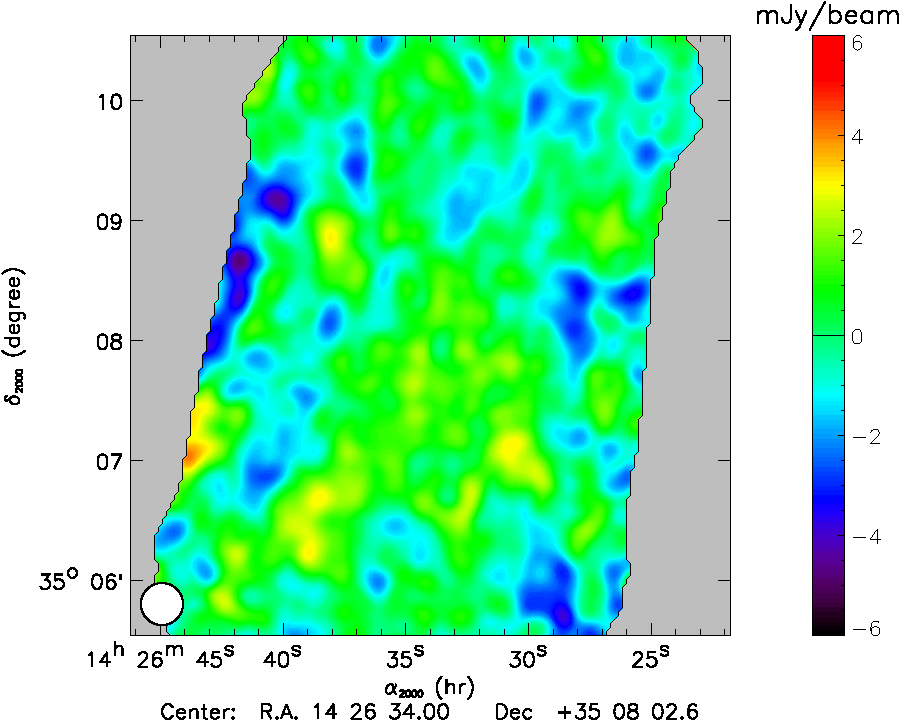
\includegraphics[width=\columnwidth]{Figure/IDCS_J1426}
\caption{Map at 140~GHz of the undetected galaxy cluster \mbox{IDCS~J1426.5+3508}.}
\label{fig:IDCS_J1426}
\end{figure}
	
	
